\documentclass[11pt,a4paper,dvipdfmx]{article}
%\documentclass[autodetect-engine,dvipdfmx-if-dvi,ja=standard]{bxjsarticle}

\usepackage[utf8]{inputenc}
\usepackage{lmodern}
\usepackage[T1]{fontenc}
\usepackage[noBBpl]{mathpazo}
%\linespread{1.05}
\usepackage{mathtools, amsmath, amssymb, amsthm}
\usepackage{amsfonts}
\usepackage{braket}
%\usepackage{amssymb}
\usepackage{url}
\usepackage{cases}

%% citation
\usepackage[longnamesfirst]{natbib}

%
\theoremstyle{plain}
\newtheorem{thm}{Thm.}[section]
\newtheorem{lem}{Lem.}[section]
\newtheorem{cor}{Cor.}[section]
\newtheorem{prop}{Prop.}[section]
\newtheorem{df}{Def.}[section]
\newtheorem{eg}{e.g.}[section]
\newtheorem{rem}{Rem.}[section]
%

\usepackage{listings,jlisting}
\lstset{%
language={python},%
basicstyle={\ttfamily\footnotesize},%ソースコードの文字を小さくする
frame={single},
commentstyle={\footnotesize\itshape},%コメントアウトの文字を小さくする
breaklines=true,%行が長くなったときの改行。trueの場合は改行する。
numbers=left,%行番号を左に書く。消す場合はnone。
xrightmargin=3zw,%左の空白の大きさ
xleftmargin=3zw,%右の空白の大きさ
stepnumber=1,%行番号を1から始める場合こうする(たぶん)
numbersep=1zw,%行番号と本文の間隔。
}

%\usepackage[dvipdfmx]{graphicx}
%% color packageとdvipdfmxは相性が悪いらしい
%% https://qiita.com/zr_tex8r/items/442b75b452b11bee8049
\usepackage{graphicx}


\usepackage[left=2cm,right=2cm,top=2cm,bottom=2cm]{geometry} %This changes the margins.
\usepackage{float}
%\author{Kyohei Okumura}
\global\long\def\T#1{#1^{\top}}

\newcommand{\id}{\textnormal{id}}
\newcommand{\R}{\mathbb{R}}
\newcommand{\N}{\mathbb{N}}
\newcommand{\Q}{\mathbb{Q}}
\newcommand{\Z}{\mathbb{Z}}
\newcommand{\C}{\mathbb{C}}
\newcommand{\mF}{\mathcal{F}}
\newcommand{\mG}{\mathcal{G}}
\newcommand{\mA}{\mathcal{A}}
\newcommand{\mB}{\mathcal{B}}
\newcommand{\mC}{\mathcal{C}}
\newcommand{\mD}{\mathcal{D}}
\newcommand{\mL}{\mathcal{L}}
\newcommand{\mM}{\mathcal{M}}
\newcommand{\mO}{\mathcal{O}}
\newcommand{\mP}{\mathcal{P}}
\newcommand{\mS}{\mathcal{S}}
\newcommand{\mT}{\mathcal{T}}
\newcommand{\mV}{\mathcal{V}}
\renewcommand{\Re}{\mathrm{Re}}
\renewcommand{\hat}{\widehat}
\renewcommand{\tilde}{\widetilde}
\renewcommand{\bar}{\overline}
\renewcommand{\epsilon}{\varepsilon}
% \renewcommand{\span}{\mathrm{span}}
\newcommand{\defi}{\stackrel{\Delta}{\Longleftrightarrow}}
\newcommand{\equi}{\Longleftrightarrow}
\newcommand{\s}{\succsim}
\newcommand{\p}{\precsim}
\newcommand{\join}{\vee}
\newcommand{\meet}{\wedge}
\newcommand{\1}{\mbox{1}\hspace{-0.25em}\mbox{l}}

\DeclareMathOperator{\Var}{Var}
\DeclareMathOperator{\Cov}{Cov}
\DeclareMathOperator{\sgn}{sgn}
\DeclareMathOperator{\Card}{Card}
\DeclareMathOperator{\supp}{supp}
\DeclareMathOperator{\Log}{Log}
\DeclareMathOperator{\spn}{span}

\newcommand{\indep}{\mathop{\perp\!\!\!\!\perp}}

\usepackage{color}
\newcommand{\kcomment}[1]{{\textcolor{blue}{#1}}}
\newcommand{\ocomment}[1]{{\textcolor{red}{#1}}}


\begin{document}
\title{SML HW2}
\author{29-176004 奥村 恭平{\footnote{E-mail: kyohei.okumura@gmail.com}
\footnote{東京大学大学院 経済学研究科 M2}
}}
\date{\today}
\maketitle

%%%%%%%%%%%%%%%%%%%%%%%%%%%%%%%%%%%%%%%%%%%%%%%%%%%%%%%%%%%

\section*{宿題1}
$\Sigma := \sigma^2 I$のガウスモデルの最尤推定量が,次のようになることを示す.
\begin{equation} \label{goal_1}
	\hat{\mu}_{ML} = \frac{1}{n}\sum_{i=1}^n x_i, \ 
	\hat{\sigma}^2_{ML} = \frac{1}{nd} \sum_{i=1}^d \sum_{j=1}^n (x_j^{(i)} - \hat{\mu}^{(i)}_{ML})(x_j^{(i)} - \hat{\mu}^{(i)}_{ML})
\end{equation}

対数尤度関数$l(\mu, \sigma^2)$は,以下のようになる.
$$
l(\mu, \sigma^2) := \sum_{i=1}^n \log q(x_i; \mu, \sigma^2) \propto \frac{nd}{2} \log \sigma^2 - \frac{1}{2 \sigma^2} \sum_{i=1}^n (x_i - \mu)^\top (x_i - \mu)
$$

最尤推定量は以下の方程式系を満たす.
\begin{numcases}
	{}
	\frac{\partial l}{\partial \mu} = 0 & \label{eq1}\\ 
	\frac{\partial l}{\partial \sigma^2} = 0 \label{eq2}& 
\end{numcases}
これを解くと,
\begin{align*}
	(\ref{eq1})
	&\equi \frac{1}{2 \sigma^2}\sum_{i=1}^n 2(x_i - \mu) = 0 \\
	&\equi \sum_{i=1}^n (x_i - \mu) = 0 \\
	&\therefore \ \hat{\mu}_{ML} = \frac{1}{n}\sum_{i=1}^n x_i
\end{align*}
\begin{align*}
	(\ref{eq2}) &\equi - \frac{nd}{2} \frac{1}{\sigma^2} + \frac{1}{2(\sigma^2)^2} \sum_{j=1}^n (x_j - \mu)(x_j - \mu)^\top  = 0 \\
	&\equi \sigma^2 = \frac{1}{nd}\sum_{j=1}^n (x_j - \mu)(x_j - \mu)^\top \\
	&\therefore \ 
	\hat{\sigma}^2_{ML} = \frac{1}{nd} \sum_{i=1}^d \sum_{j=1}^n (x_j^{(i)} - \hat{\mu}^{(i)}_{ML})(x_j^{(i)} - \hat{\mu}^{(i)}_{ML})
\end{align*}
となり,所定の結果(\ref{goal_1})を得る.
\qed


%%%%%%
\newpage
\section*{宿題2}
$$
\mu_1 = \left(
\begin{matrix}
	2  \\
	0
\end{matrix}
\right), \ 
\mu_2 = \left(
\begin{matrix}
	-2  \\
	0
\end{matrix}
\right), \ 
\Sigma_1 = \Sigma_2 = \Sigma =\left(
\begin{matrix}
	9 - 8 \cos^2 \beta & 8 \sin \beta \cos \beta  \\
	8 \sin \beta \cos \beta & 9 - 8 \sin^2 \beta 
\end{matrix}
\right), \
p(y=1) = p(y=2) = 1/2
$$

まず,
$$
\Sigma^{-1} = 
\left(
\begin{matrix}
	1 - \frac{8}{9} \sin^2 \beta & - \frac{8}{9} \sin \beta \cos \beta  \\
	- \frac{8}{9} \sin \beta \cos \beta  & 1 - \frac{8}{9} \cos^2 \beta 
\end{matrix}
\right)
$$
である.データから決定境界を推定した場合の推定された決定境界の式は以下のようになる.
$$
\hat{a}^\top x + \hat{b} = 0, 
\text{where } \hat{a}:=\hat{\Sigma}^{-1}(\hat{\mu_1} - \hat{\mu_2}), \hat{b}:= -\frac{1}{2}(\hat{\mu}_1^\top \hat{\Sigma}^{-1} \hat{\mu}_1 - \hat{\mu}_2^\top \hat{\Sigma}^{-1} \hat{\mu}_2) + \log \frac{n_1}{n_2}
$$
サンプルサイズ$n$が十分大きいとき,大数の法則・最尤推定量の一致性より,
$$
\hat{a} \to^p \Sigma^{-1}(\mu_1 - \mu_2) = 
\left(
\begin{matrix}
	4 - \frac{32}{9} \sin^2 \beta \\
	-\frac{32}{9}\sin \beta \cos \beta
\end{matrix}
\right)
$$
$$
\hat{b} \to^p -\frac{1}{2}(\mu_1^\top \Sigma^{-1} \mu_1 - \mu_2^\top \Sigma^{-1} \mu_2) + \log \frac{n \cdot p(y=1)}{n \cdot p(y=2)} = 0
$$

よって,決定境界の式は,漸近的に
$$
\left( 4 - \frac{32}{9} \sin^2 \beta \right) x_1 - \left( \frac{32}{9} \sin \beta \cos \beta \right)x_2 = 0
$$
となる.


%%%%%%
\section*{宿題3}
Pythonを用いて実装した.$n := 600, \alpha := 0.1$としてシミュレーションを行った際の図を載せる.黒い直線が,データから推定された決定境界を表している.

\begin{figure}[H]
  \centering
    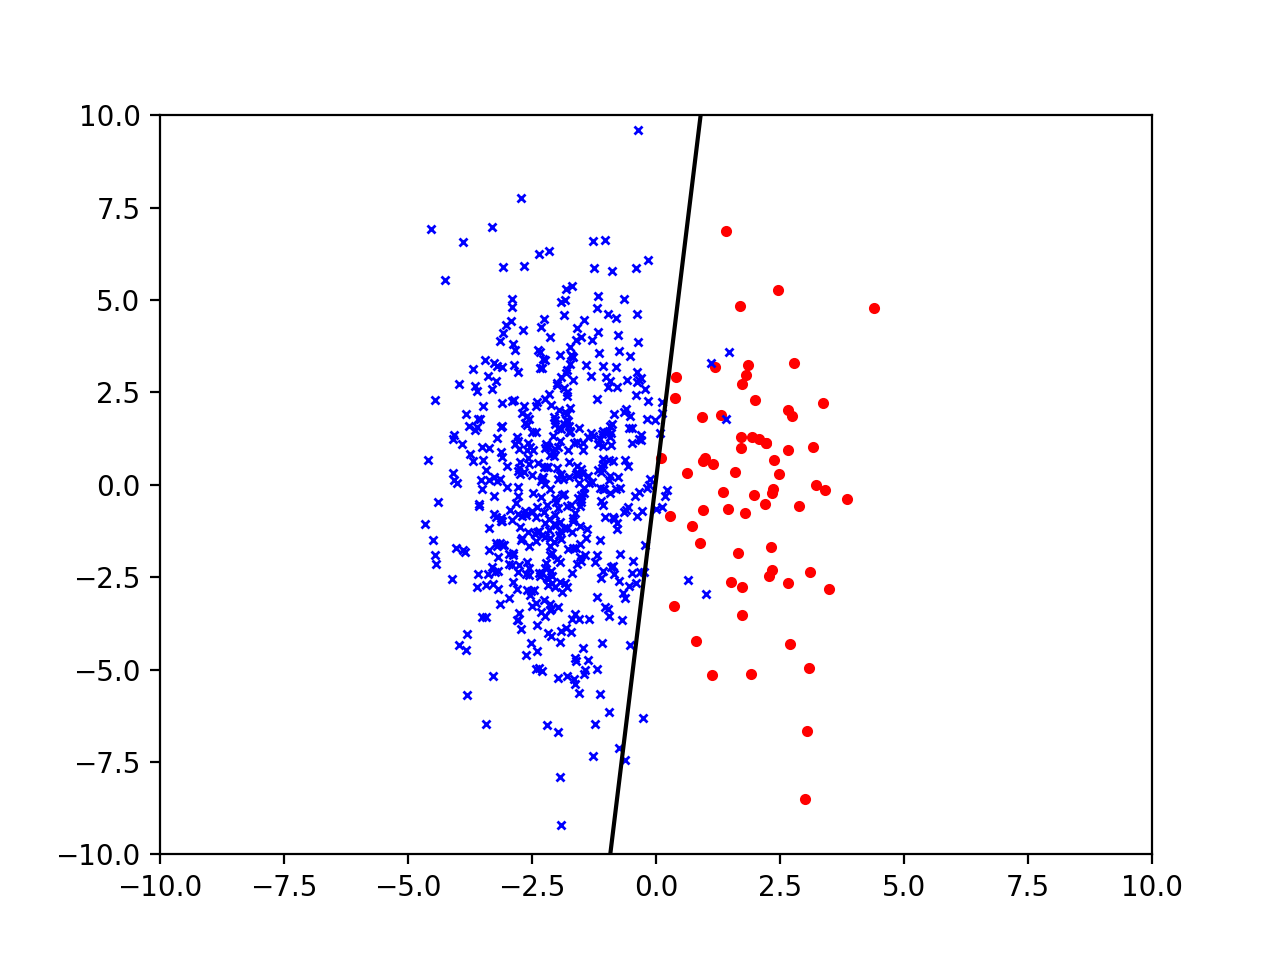
\includegraphics[height=8cm]{image/Figure_1.png}
    \caption{\footnotesize $n := 600, \alpha := 0.1$}
    \label{fig:prob1}
\end{figure}

以下,用いたコード.
\begin{lstlisting}[caption=Fisher]
import numpy as np
from numpy.random import randn, rand
import matplotlib.pyplot as plt


def gen(n=600, alpha=0.1):
# data generation
    n1 = np.sum(rand(n, 1) < alpha)
    n2 = n - n1
    x1 = np.concatenate([randn(1, n1) + 2, 3 * randn(1, n1)])
    x2 = np.concatenate([randn(1, n2) - 2, 3 * randn(1, n2)])
    
    return x1, x2


def plot(x1, x2, line=None):
    x, y = x1
    plt.plot(x, y, 'ro', ms=3, label='class1')
    x, y = x2
    plt.plot(x, y, 'bx', ms=3, label='class2')
    
    if not (line is None):
            plt.plot(line[0], line[1], 'k-', ms=5)

    plt.xlim(-10, 10)
    plt.ylim(-10, 10)
    
    plt.show()


def fisher(x1, x2):
    x1 = x1.T
    x2 = x2.T
    n1 = x1.shape[0]
    n2 = x2.shape[0]
    n = n1 + n2
    
    # dimension
    DIM = x1.shape[1]
    
    
    # average
    mean1 = np.mean(x1, axis=0)
    mean1 = mean1.reshape(DIM, 1)
    mean2 = np.mean(x2, axis=0)
    mean2 = mean2.reshape(DIM, 1)
    
    # covariance
    sample_cov_1 = np.zeros((DIM, DIM))
    sample_cov_2 = np.zeros((DIM, DIM))
    for x_i in x1:
        x_i = x_i.reshape(DIM, 1)
        sample_cov_1 += np.dot((x_i - mean1), (x_i - mean1).T)
        sample_cov_1 = sample_cov_1 / n1
    for x_i in x2:
        x_i = x_i.reshape(DIM, 1)
        sample_cov_2 += np.dot((x_i - mean2), (x_i - mean2).T)
        sample_cov_2 = sample_cov_2 / n2
    sample_cov = (n1/n) * sample_cov_1 + (n2/n) * sample_cov_2
    
    sample_cov_inv = np.linalg.inv(sample_cov + 0.000001 * np.eye(DIM))
    
    a = np.dot(sample_cov_inv, (mean1 - mean2))
    if (n1 - n2 > 1e-10):
        b = -0.5 * (np.dot(mean1.T, np.dot(sample_cov_inv, mean1)) - np.dot(mean2.T, np.dot(sample_cov_inv, mean2))) + np.log(n1/n2)
    else:
        b = -0.5 * (np.dot(mean1.T, np.dot(sample_cov_inv, mean1)) - np.dot(mean2.T, np.dot(sample_cov_inv, mean2)))
    b = b.reshape(1)

    return a, b



def line_est(a, b, x):
    if abs(a[1]) > 1e-10:
        c = - a[0]/a[1]
        d = - b/a[1]
    return [x, c*x+d]


if __name__ == '__main__':
    x1, x2 = gen(n=600, alpha=0.1)
    a, b = fisher(x1, x2)
    x = np.linspace(-10, 10, 3000)
    l = line_est(a, b, x)
    plot(x1, x2, l)
\end{lstlisting}


%%%%%%
\section*{宿題4}
Octaveで末尾のコードを実行し,コンソールで混同行列を表示した.その画像を添付する.
\begin{figure}[H]
  \centering
    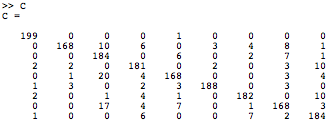
\includegraphics[height=5cm]{image/c.png}
    \caption{\footnotesize 混同行列}
    \label{fig:prob4}
\end{figure}


(pythonのコードを貼る設定でmatlabのコードを貼っているため,latexでの表示が少しおかしくなっています.)
\begin{lstlisting}[caption=digits]
clear all
load digit.mat X T
[d,n,nc] = size(X);

nc = 9;
S = zeros(d,d);
for c = 1:nc
  mu(:,c) = mean(X(:,:,c), 2);
  S = S + cov(X(:,:,c)')/nc;
end
invS = inv(S);

for ct = 1:nc
  for c = 1:nc
    muc = mu(:,c);
    t=T(:,:,ct);
    p(ct,:,c) = t' * invS * muc - muc' * invS * muc /2;
  end
end

[pmax P] = max(p, [], 3);
for ct = 1:nc
  for c = 1:nc
    C(ct, c) = sum(P(ct,:)==c);
  end
end
\end{lstlisting}



\end{document}